%!TEX root = project.tex

\chapter*{About this project}
\paragraph{Abstract}
A dynamic web app that creates curated playlists based on multiple user's music preferences using Spotify. Built with React, Flask, Python, Node.js, Mocha, AWS and Mongo.

\paragraph{Authors}
\begin{flushleft}
	Eddie Eldridge
	
	Danielis Joniskis
	
	Keith Higgins
	
	Three students from the Galway-Mayo Institute of Technology
\end{flushleft}



\chapter{Introduction}
The introduction should be about three to five pages long.
Make sure you use references~\cite{einstein}
\begin{flushleft}
	Context for the Project.
	
	
	Objectives of the Project.
	
	
	Is the reader 100 percent of what the project is all about 
\end{flushleft}


\chapter{Context}
\begin{itemize}
\item Provide a context for your project.
\item Set out the objectives of the project
\item Briefly list each chapter / section and provide a 1-2 line description of what each section contains.
\item List the resource URL (GitHub address) for the project and provide a brief list of the main elements at the URL.
\end{itemize}

\section{Filler}
Lorem ipsum dolor sit amet, consectetur adipiscing elit. Etiam mi enim, interdum ut elit lobortis, bibendum tempus diam. Etiam turpis ex, viverra tristique finibus nec, feugiat at metus. Curabitur tempus gravida interdum. Donec ac felis a lorem scelerisque elementum. Vestibulum sit amet gravida tortor, a iaculis orci. Nam a molestie augue. Curabitur malesuada odio at mattis molestie. In hac habitasse platea dictumst. Donec eu lectus eget risus hendrerit euismod nec at orci. Praesent porttitor aliquam diam, eu vestibulum nisl sollicitudin vel. Nullam sed egestas mi.

Quisque vel erat a justo volutpat auctor a nec odio. Sed rhoncus augue sit amet nisl tincidunt, vitae cursus tellus efficitur. Class aptent taciti sociosqu ad litora torquent per conubia nostra, per inceptos himenaeos. Pellentesque et auctor dui. Fusce ornare odio ipsum, et laoreet mi molestie sed. Cras at massa sit amet ipsum gravida aliquam. Nulla suscipit porta imperdiet. Fusce eros neque, bibendum sit amet consequat non, pulvinar quis ipsum.

\subsection{More filler}
Donec fermentum sapien ac rhoncus egestas. Nullam condimentum condimentum eros sit amet semper. Nam maximus condimentum ligula. Praesent faucibus in nisi vitae tempus. Sed pellentesque eleifend ante, ac malesuada nibh dapibus nec. Phasellus nisi erat, pulvinar vel sagittis sed, auctor et magna. Quisque finibus augue elit, consequat dignissim purus mollis nec. Duis ultricies euismod tortor, nec sodales libero pellentesque et. Interdum et malesuada fames ac ante ipsum primis in faucibus.

Donec id interdum felis, in semper lacus. Mauris volutpat justo at ex dignissim, sit amet viverra massa pellentesque. Suspendisse potenti. Praesent sit amet ipsum non nibh eleifend pretium. In pretium sapien quam, nec pretium leo consequat nec. Pellentesque non dui lacus. Aenean sed massa lacinia, vehicula ante et, sagittis leo. Sed nec nisl ac tellus scelerisque consequat. Ut arcu metus, eleifend rhoncus sapien sed, consequat tincidunt erat. Cras ut vulputate ipsum.

Curabitur et efficitur augue. Proin condimentum ultrices facilisis. Mauris nisi ante, ultrices sed libero eget, ultrices malesuada augue. Morbi libero magna, faucibus in nunc vitae, ultricies efficitur nisl. Donec eleifend elementum massa, sed eleifend velit aliquet gravida. In ac mattis est, quis sodales neque. Etiam finibus quis tortor eu consequat. Nullam condimentum est eget pulvinar ultricies. Suspendisse ut maximus quam, sed rhoncus urna.

\section{Filler}
Phasellus eu tellus tristique nulla porttitor convallis. Vestibulum ac est eget diam mollis consectetur. Donec egestas facilisis consectetur. Donec magna orci, dignissim vel sem quis, efficitur condimentum felis. Donec mollis leo a nulla imperdiet, in bibendum augue varius. Quisque molestie massa enim, vitae ornare lacus imperdiet non. Donec et ipsum id ante imperdiet mollis. Nullam est est, euismod sit amet cursus a, feugiat a lectus. Integer sed mauris dolor.

Mauris blandit neque tortor, consequat aliquam nisi aliquam vitae. Integer urna dolor, fermentum ut iaculis ut, semper eu lacus. Curabitur mollis at lectus at venenatis. Donec fringilla diam ac risus imperdiet suscipit. Aliquam convallis quam vitae turpis interdum, quis pharetra lacus tincidunt. Nam dictum maximus lectus, vitae faucibus ante. Morbi accumsan velit nec massa tincidunt porttitor. Nullam gravida at justo id viverra. Mauris ante nulla, eleifend vitae sem vitae, porttitor lobortis eros.

Cras tincidunt elit id nisi aliquam, id convallis ex bibendum. Sed vel odio fringilla, congue leo quis, aliquam metus. Nunc tempor vehicula lorem eu ultrices. Curabitur at libero luctus, gravida lectus sed, viverra mi. Cras ultrices aliquet elementum. Pellentesque habitant morbi tristique senectus et netus et malesuada fames ac turpis egestas. Sed metus ante, suscipit sit amet finibus ut, gravida et orci. Nunc est odio, luctus quis diam in, porta molestie magna. Interdum et malesuada fames ac ante ipsum primis in faucibus. Mauris pulvinar lacus odio, luctus tincidunt magna auctor ut. Ut fermentum nisl rhoncus, tempus nulla eget, faucibus tortor. Suspendisse eu ex nec nunc mollis pulvinar. Nunc luctus tempus tellus eleifend porta. Nulla scelerisque porttitor turpis porttitor mollis.

Duis elementum efficitur auctor. Nam nisi nulla, fermentum sed arcu vel, posuere semper dui. Fusce ac imperdiet felis. Aenean quis vestibulum nisl. Integer sit amet tristique neque, at suscipit tortor. Morbi et placerat ante, vel molestie dui. Vivamus in nibh eget massa facilisis accumsan. Nunc et purus ac urna fermentum ultrices eget sit amet justo. Class aptent taciti sociosqu ad litora torquent per conubia nostra, per inceptos himenaeos. Cras elementum dui nunc, ac tempor odio semper et. Ut est ipsum, sollicitudin eleifend nisl eu, scelerisque cursus nunc. Nam at lectus vulputate, volutpat tellus vel, pharetra mauris. Integer at aliquam massa, at iaculis sem. Morbi nec imperdiet odio. In hac habitasse platea dictumst.

Mauris a neque lobortis, venenatis erat ut, eleifend quam. Nullam tincidunt tellus quis ligula bibendum, a malesuada erat gravida. Phasellus eget tellus non risus tincidunt sagittis condimentum quis enim. Donec feugiat sapien sit amet tincidunt fringilla. Vivamus in urna accumsan, vehicula sem in, sodales mauris. Aenean odio eros, tristique non varius id, tincidunt et neque. Maecenas tempor, ipsum et sollicitudin rhoncus, nibh eros tempus dolor, vitae dictum justo massa in eros. Proin nec lorem urna. In ullamcorper vitae felis sit amet tincidunt. Maecenas consectetur iaculis est, eu finibus mi scelerisque et. Nulla id ex varius, ultrices eros nec, luctus est. Aenean ac ex eget dui pretium mattis. Ut vitae nunc lectus. Proin suscipit risus eget ligula sollicitudin vulputate et id lectus.


\chapter{Methodology}
About one to two pages.
Describe the way you went about your project:
\begin{itemize}
\item Agile / incremental and iterative approach to development. Planning, meetings.
\item What about validation and testing? Junit or some other framework.
\item If team based, did you use GitHub during the development process.
\item Selection criteria for algorithms, languages, platforms and technolo-gies.
\end{itemize}
Check out the nice graphs in Figure \ref{tikz:graphs}, and the nice diagram in Figure \ref{tikz:mydiagram}.

\begin{figure}
  \centering
  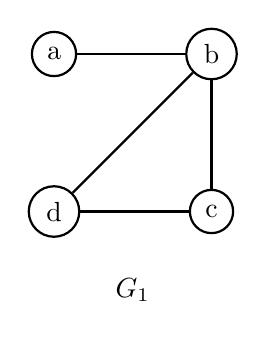
\begin{tikzpicture}
  \begin{scope}[every node/.style={circle,thick,draw}]
  \node (a) at (0,2) {a};
  \node (b) at (2,2) {b};
  \node (c) at (2,0) {c};
  \node (d) at (0,0) {d};
  \end{scope}
  \begin{scope}[every edge/.style={draw=black,thick}]
  \path (a) edge (b);
  \path (b) edge (c);
  \path (b) edge (d);
  \path (c) edge (d);
  \end{scope}
  \node () at (1,-1) {$G_1$};
  \end{tikzpicture}
  \hspace{1.5cm}
  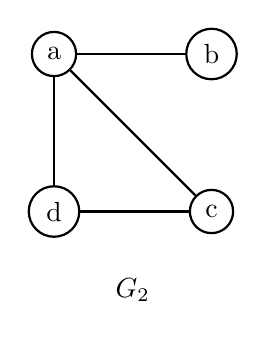
\begin{tikzpicture}
  \begin{scope}[every node/.style={circle,thick,draw}]
  \node (1) at (0,2) {a};
  \node (2) at (2,2) {b};
  \node (3) at (2,0) {c};
  \node (4) at (0,0) {d};
  \end{scope}
  \begin{scope}[every edge/.style={draw=black,thick}]
  \path (1) edge (2);
  \path (1) edge (3);
  \path (1) edge (4);
  \path (3) edge (4);
  \end{scope}
  \node () at (1,-1) {$G_2$};
  \end{tikzpicture}
  \caption{Nice pictures}
  \label{tikz:graphs}
\end{figure}


\begin{figure}
  \centering
  \begin{tikzpicture}[node distance=6cm]
  \node (a) [rect] {A Big Blue Block};
  \node (b) [oval, right of=a] {And His Oval Friend};
  \draw [line] (a) -- (b);
  \end{tikzpicture}
  \caption{Nice pictures}
  \label{tikz:graphs}
\end{figure}


\chapter{Technology Review}
About seven to ten pages.
\begin{itemize}
\item Describe each of the technologies you used at a conceptual level. Standards, Database Model (e.g. MongoDB, CouchDB), XMl, WSDL, JSON, JAXP.
\item Use references (IEEE format, e.g. [1]), Books, Papers, URLs (timestamp) – sources should be authoritative. 
\end{itemize}

\section{AWS}
Amazon Web Services offers reliable, scalable, and inexpensive cloud computing services.

\begin{minted}{xml}
<this>
  <looks lookswhat="good">
    Good
  </looks>
</this>
\end{minted}

\section{MongoDB}
MongoDB is an open-source, document database designed for ease of development and scaling. MongoDB stores data in JSON-like documents, which makes the database very flexible and scalable.\cite{w3schools}

\section{Flask}
Flask is a microframework for Python.

\section{Python}
Python is a programming language that lets you work more quickly and integrate your systems more effectively.

\section{Mocha}
Mocha is a JavaScript test framework running on Node.js. Mocha tests run serially, allowing for flexible and accurate reporting

\section{React}
React is a JavaScript library for building user interfaces. React is developed by Facebook. It is a tool for building UI components. React uses Babel to convert JSX (JavaScript XML) into JavaScript. Babel is a JavaScript compiler that can translate markup or programming languages into JavaScript. With Babel, you can use the newest features of JavaScript (ES6 - ECMAScript 2015). \cite{w3schools}

\chapter{System Design}
As many pages as needed.
\begin{itemize}
\item Architecture, UML etc. An overview of the different components of the system. Diagrams etc… Screen shots etc.
\end{itemize}

\begin{table}[h]
  \centering
  \begin{tabular}{x{2cm}p{3cm}}
    \toprule \\
    Column 1 & Column 2 \\
    \midrule \\
    Rows 2.1 & Row 2.2 \\
    \bottomrule
  \end{tabular}
  \caption{A table.}
  \label{table:mytable}
\end{table}

\chapter{System Evaluation}
In this chapter, we will discuss many aspects of the software. We will break the evaluation down into 4 headings.
\begin{itemize}
  \item Robustness - How well the software can deal with problems, it's ability to handle change etc.
  \item Performance - Space and time complexity of the software, responsiveness etc.
  \item Testing - A general overview of the testing approach taken
  \item Overall evaluation - Where the project succeeded/failed, limitations in our approach and technologies etc.
  \end{itemize}

  \subsection{Robustness}
  Robustness in regards to software can be defined as the ability of the software to cope with errors during execution and cope with erroneous input. Measuring the robustness of a system is difficult 
  as no system can be considered completely robust. However, there are certain methodologies and practices we can implement to increase the robustness of a system. {\textit{Behdis Eslamnour and Shoukat Ali}} discuss these metrics in their paper entitled {\textit{Measuring robustness of computing systems}}\cite{SoftwareRobustness}
  Some of these proposed metrics include
    \newline
    \begin{itemize}
      \item Error Handling/Error Catching
      \item Time between failures and time between recovery
    \end{itemize}

    \subsection{Error Handling}
    Error handling refers to how a system handles errors should they occur. This can be as simple as logging the error in the console to rolling back the system to a previous stable release.
    It is a vital aspect for any system from both the perspective of the user and developer. As a developer, implementing proper error handling and catching is an important aspect of development
    as it enables the developer to work more effectively and efficiently as less time is spent fixing and locating the cause of bugs if proper error handling is done pre-emptively.

    For the user, it's vital that error handling is done correctly as incorrect error handling can have a significant impact on the end-users experience of the system/software. For example, if a user
    attempts to login to a system and their login details are incorrect, a meaningful way of handling this error would be to notify the user that their login details are incorrect. If this is not done, 
    the end user won't understand what's happening and why they can't use the system and as a result of this will become frustrated/unhappy with the service. As such it's important to make sure any critical
    problems such as this are caught and handled in an appropriate manner. However, it's also important to remember that complete robustness can not be achieved and as such one must try and figure out the 
    most important and likely errors to handle. When making these decisions, one can consider many factors when deciding what errors to handle such as the risk of not handling the error (application crashing, unexpected behaviour, potential security risk, loss of data etc.)
    , how much time will be required to handle the error and the likelihood of the error occuring. However, as mentioned above complete robustness can not be achieved as to even consider the above factors,
    one must have the foresight to see that the error will occur in the firstplace.

    Below I will discuss some error handling that occured in our project and how it contributed to the overall robustness of the system.
    
    \textbf{Example 1 - Login/Register} 
    In the image below we can see how error handling and error catching can produce meaningful output and guide the user through login/register scenario of our application

    ---- user login diagram here ----

    \textbf{Example 2 - Authentication with Spotify}
    In the image below we can see how error handling and error catching can produce meaningful output and guide the user through authenticating our applicatin with Spotify.

    --- authentication diagram here ----


    The above error handling was done on both the server and client-side of the application. Both Python, MongoDB and Pythn provide useful tools for error handling/catching.
    Some examples include \textit{Error boundaries} in React, \textit{Try/Catch/Raise statements} and \textit{Schema validation} in MongoDB.

    \begin{itemize}
      \item Error Boundaries - Error boundaries are React components that catch JavaScript errors anywhere in their child component tree, log those errors, and display a fallback UI instead of the component tree that crashed.
      \item Try/Catch/Raise statemetns - These commonly found in most programming languages and Python is no exception. We used these to catch certain errors such as HTTPErrors, null value errors, MongoDB errors and many others.
      \item Schema Validation - To ensure the data being passed into the Mongo database was in the correct format, we used a JSON Schema to validate our inputs against before passing it to Mongo. In the below example, we can see that for a user 
      to be validated correctly, the minimum required properties are an email and password. This ensures that user's cant create accounts without these two required properties.
      \begin{minted}{JSON}
      user_schema = {
        "type": "object",
        "properties": {
            "name": {
                "type": "string",
            },
            "email": {
                "type": "string",
                "format": "email"
            },
            "password": {
                "type": "string",
            },
            "spotifyUsername": {
                "type": "string",
            },
          
        },
        "required": ["email", "password"],
        "additionalProperties": False
      }
      \end{minted}
      
    \end{itemize}

    \subsection{Time between failures and time between recovery}
    Time between failures and time between recovery are too very useful metrics in determining the robustness of a system. Systems that have a short mean time between failures and mean time between recovery
    either have excellent error handling or are designed in such a way that errors do not occur frequently. A good way of measuring this could be 
    the downtime of your application over the course of a year. For example, on average, the top 50 e-commerce websites experienced 99.03\% uptime. Over a year, 99.03\% uptime would result in 3 days 15 hours and 39 minutes of downtime. 32 of
    these websites experienced 99.99\% uptime. 9 out of 10 of users encountering a website that is not up will choose to use a competitors website \cite{WebsiteDowntimeStats}. From these statistics, we can see that time between failures anre time between recovery are extremely important aspects to 
    any system/application. As such, they can be very helpful metrics when trying to measure the robustness of an application. 

    In regards to WePick's failure and recovery time, since the project was hosted on AWS' Elastic Beanstalk, there have been little to no outages as due 
    to the continous integration solution integrated upon deployment, it was not possible for broken code to be deployed as any code proposed to be deployed had 
    to first pass tests that were outlined by Travis CI and any problems that did arrive were dealt with quickly as Travis instantly notified us of any problems which we were 
    able to fix quickly and promptly.



\chapter{Conclusion}
About three pages.

\begin{itemize}
\item Briefly summarise your context and ob-jectives (a few lines).
\item Highlight your findings from the evalua-tion section / chapter and any opportuni-ties identified.
\end{itemize}

